
% Andrew G. West - prop_spec.tex
% Main LaTeX file for CIS400/401 Project Proposal Specification
%
% Once built and in PDF form this document outlines the format of a project proposal. However, in raw (.tex) form, we also try to comment on some basic LaTeX technique. This is not intended to be a LaTeX tutorial, instead just (1) a use-case thereof, and (2) a template for your own writing.

	% AW - Ordinarily we'd begin by specifying some broad document properties like font-size, page-size, margins, etc. -- We have done this (and much more) for you by creating a 'style file', which the 'documentclass' command references.
\documentclass{sig-alternate}
 
	% AW - These 'usepackage' commands are a way of importing additional LaTeX styles and formattings that aren't part of the 'standard library'
\usepackage{mdwlist}
\usepackage{url}
\usepackage{hyperref}

\begin{document} 

\title{CIS400/401 Final Report - Designing Rhythm Game Interfaces for Touchscreen Devices}
\subtitle{Dept. of CIS - Senior Design 2011-2012}
\numberofauthors{2}
\author{
\alignauthor Philip H. Peng \\ \email{pengp@stwing.upenn.edu} \\ Univ. of Pennsylvania \\ Philadelphia, PA
\alignauthor Stephen H. Lane \\ \email{shlane@cis.upenn.edu} \\ Univ. of Pennsylvania \\ Philadelphia, PA}
\date{}
\maketitle

\begin{abstract}
\textit{As touchscreen devices become increasingly popular, rhythm games and other interactive software applications are expected to support touch-driven user interfaces. This study focused on the evaluation of the timing accuracy and game enjoyability of various rhythm game interface designs for touchscreen devices. This was accomplished through the development of a rhythm game prototype for Android tablets, ''Beats2 Prototypes''. The prototype app demonstrated various gameplay user interfaces and collected usage data for quantitative and qualitative comparisons.}
\end{abstract}

\section{Introduction}
\label{sec:intro}
Over the past few years, touchscreen devices have become increasingly common in the consumer market. According to a report in the March 2010 publication of \textit{Information Display}, consumer-device manufacturers are rapidly adopting touch-input technologies, with revenues increasing \textit{10x} and unit production \textit{3x} faster than the display industry~\cite{information_display}. With the adoption of this new input paradigm comes the natural expectation of increased software support for new touch-focused interfaces, allowing for faster and more natural human-device interactions~\cite{hayes_thesis}.\\

One area that touchscreen support can be leveraged is in the design of rhythm games. A \textit{touchscreen} is a specialized display that receives user input through physical contact from a finger or stylus. \textit{Rhythm games} are a genre of music-based games in which the player performs specific actions in response to audio and visual cues. Rhythm games often focus the player's beat recognition abilities, aided through visual patterns that match the rhythm of the song. These visual patterns consist of a series of \textit{note} objects that appear or move across the screen. Interaction with these notes would typically involve hand actions occuring in the \textit{hitbox} area, a pre-defined area for interaction. In non-touchscreen rhythm games, such actions may be the pressing of a button; in a touchscreen scenario, such actions would be either \textit{soft button} touches, defined as virtual buttons interacted by through tap, or \textit{touch-input gestures}, defined as touch events with predefined timing and path properties. The performance of the player is reflected by their \textit{timing accuracy}, measured by the time difference between the timestamp of the touch event and the expected time for that note.\\

The success of a rhythm game depends on two main factors: 1) game mechanics that allow players to best maximize their timing accuracy, and 2) a gameplay experience that is perceived as enjoyable. Both factors are strongly influenced by the gameplay's \textit{interface design}, defined as the placement and movement patterns of the game's note and tapbox elements. In this study, gameplay with a specific style of interface design is referred to as a rhythm game \textit{Mode}. The interface designs must also be designed to accomodate to the input method of the hardware it will be applied to. In this study, the target hardware were large touch-screen devices such as multi-touch tablets running the Android OS. Through the development of an Android rhythm game prototype and collection of user gameplay data and feedback, this study compared the timing accuracy and game enjoyability of various different rhythm game interfaces for touchscreen devices.

\section{Related Work}
\label{sec:related_work}

\noindent \textbf{Wiimote + Dance Game}

In their study, ''Understanding Visual Interfaces for the Next Generation of Dance-Based Rhythm Video Games,'' Charbonneau et al. presented their experimental study of comparing game interfaces for \textit{RealDance}, a dancing game prototype that uses the Wiimote. Three interfaces were compared: ''Timeline'', ''Motion Lines'', and ''Beat Circles.'' The results of their studies showed that both ''Motion Lines'' and ''Beat Circles'' were significantly more efficient than the traditional ''Timeline'' interface in dance games~\cite{realdance}.\\

\noindent \textbf{External Multi-Touch Panel + Turn-based Strategy Game}

In their study, ''A Study on Multi-Touch Interaction for Game,'' Yong-Chul Kwon and Won-Hyung Lee created a multi-touch panel using FTIR technology and tested ot with a turn-based strategy game. In doing so, they created guidelines for multi-touch user interface designs and also argues that touch interfaces can be more comfortable and sensitive than traditional mouse and keyboard input given that the game interface is designed for multi-touch technology~\cite{tbs_game}. \\

\noindent \textbf{iPad + Real-Time Strategy Game}

In their study, ''One-handed interface for multitouch-enabled real-time strategy games,'' Crenshaw et al. designed a new touch-based interface for single-handed usage of large-sized touch devices. They first designed a real-time strategy game with a touch-based interface and surveyed participants with it. Their study showed that porting traditional desktop games to iOS require the development of a user interface specifically aimed at touchscreen interfaces.They argue that well designed multi-touch user interfaces can lead to faster and more accurate response times due to the larger area and less targetting precision required of gestures over traditional buttons~\cite{rts_game}.

\section{Study Overview}
\label{sec:study_overview}

This study compared rhythm game interfaces through the following three stages:
\begin{enumerate}
	\item \textit{Design} various simplified rhythm game interfaces with categorized properties\vspace{-3pt}
	\item \textit{Prototype} app development of a rhythm game that test the various interfaces\vspace{-3pt}
	\item \textit{Evaluation} of the interfaces through collecting user data and feedback\vspace{-3pt}
\end{enumerate}

\subsection{Design}
\label{subsec:study_overview}
In the \textit{Design} stage of the study, existing commercial rhythm games for various hardware platforms were analyzed and categorized based on common game interface properties. These properties were then used to create simplified rhythm game interfaces. \\

\noindent \textbf{Designs}

The results of analyzing commercial rhythm games are shown in Figure~\ref{fig:interface_analysis} in the \textit{Appendix}. Based on the generalized styles from the analysis, eight simplified interface designs were drafted and categorized as shown in Figure~\ref{fig:demo_interfaces} in the \textit{Appendix}. These interface designs were defined based on 1) the mobility of tapbox and note elements, and 2) the movement behaviours of elements within game area.\\

Three element mobility categories were chosen for the interface designs:
\begin{enumerate}
	\item Moving notes and fixed hitboxes\vspace{-3pt}
	\item Moving hitboxes and fixed notes\vspace{-3pt}
	\item Fixed notes and fixed hitboxes\vspace{-3pt}
\end{enumerate}\vspace{+6pt}

Four movement behaviour categories were chosen for the interface designs:
\begin{enumerate}
	\item Top to bottom\vspace{-3pt}
	\item Centre to corners\vspace{-3pt}
	\item Corner to centre\vspace{-3pt}
	\item Fixed grid points\vspace{-3pt}
\end{enumerate}\vspace{+6pt}

\noindent \textbf{Comparisons}

These eight interface designs encompass the majority of interface designs used by the rhythm games analysied in Figure~\ref{fig:interface_analysis}. Mode \#1 closely matches all the rhythm games under the ''Falling Notes'' style, particularly \textit{Dance Dance Revolution}. Mode \#2 is similar to the games under the \textit{Spreading Notes} style but more emphasized in the spreading aspect. In those games, objects approach from a central area in the horizon up top to a row near the bottom; in Mode \#2, the objects approach from the horizon in the centre of the screen to the four corners. Mode \#3 is similar to \textit{Gitaroo Man Lives!}'s ''Focusing Notes'' style but with four focus points instead of one. Mode \#4 closely matches \textit{jubeat}'s ''Grid'' style. Mode \#5 matches \textit{DJMax Technika}'s ''Sliding Hitbox'' style. Mode \#8 is similar to \textit{Osu! Tatakae! Ouendan!}'s ''Appearing'' style but restricts objects into a grid instead of allowing any location. This was done to reduce the complexity of the game and the player's possible reaction delay from an object appearing in an unexpected location.\\

There are currently no rhythm game with an interface similar to Mode \#6 nor \#7; however, the two styles were included as the reverses of \#2 and \#3 respectively. The ''Streaming Notes'' and ''Sliding Cursor'' styles were not covered in this study. This is because 1) they only operate on one dimension, and 2) the complexity of their gameplay comes from visual recognition of the object subtypes, a factor that is eliminated from this study through only using a single graphic for all notes objects and a single graphic for all hitbox objects.\\

\subsection{Prototype}
\label{subsec:study_overview}

\begin{figure}[htb!]
	\begin{center}
		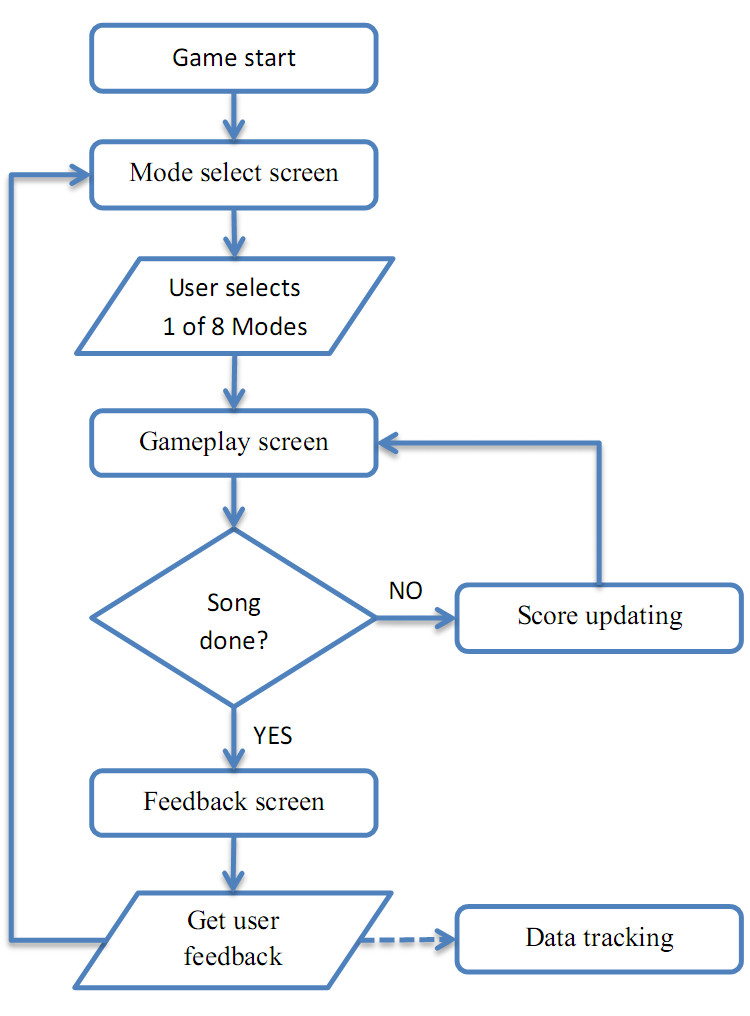
\includegraphics[width=1\linewidth]{figure_prototype_gameflow}
	\end{center}
	\vspace{-12pt}
	\caption{Gameflow diagram for the prototype app, ''Beats2 Prototypes''.}
	\label{fig:prototype_gameflow}
\end{figure}

In the \textit{Prototyping} stage of the study, the designed rhythm game prototype was created implementing the designs drafted in the previous \textit{Design} stage as eight selectable ''Modes''. Figure~\ref{fig:prototype_gameflow} shows the overall gameflow diagram of the final prototype app, ''Beats2 Prototypes''. The following are more detailed descriptions of each stage: \\

\newpage
\noindent \textbf{Game Start}

\begin{figure}[htb!]
	\begin{center}
		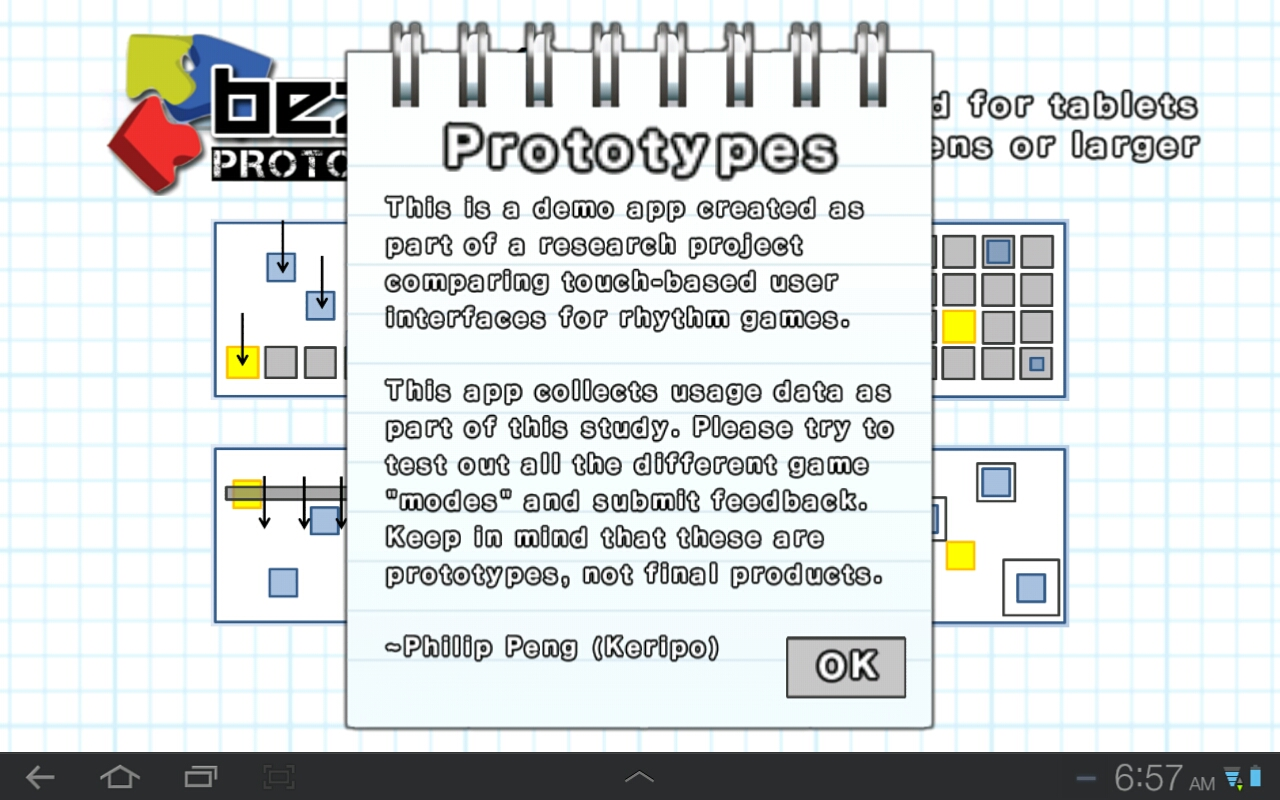
\includegraphics[width=1\linewidth]{figure_screenshot_disclaimer}
	\end{center}
	\vspace{-12pt}
	\caption{Screenshot of the data collection message.}
	\label{fig:screenshot_disclaimer}
\end{figure}

The prototype app is an Android app that can be launched from the Android tablet or phone's apps list. It was written for the cross-platform \textit{Unity3} game engine (see the \textit{Technical Resources} section for more details), so a \textit{Unity}-branded splash screen will display on start. After the splash screen, a short message will appear notifying the user than s/he is participating in a study which will collect usage data from them (see Figure~\ref{fig:screenshot_disclaimer}). After closing the disclaimer, the user will be at the ''Mode Select'' screen. \\

\noindent \textbf{Mode Select}

\begin{figure}[htb!]
	\begin{center}
		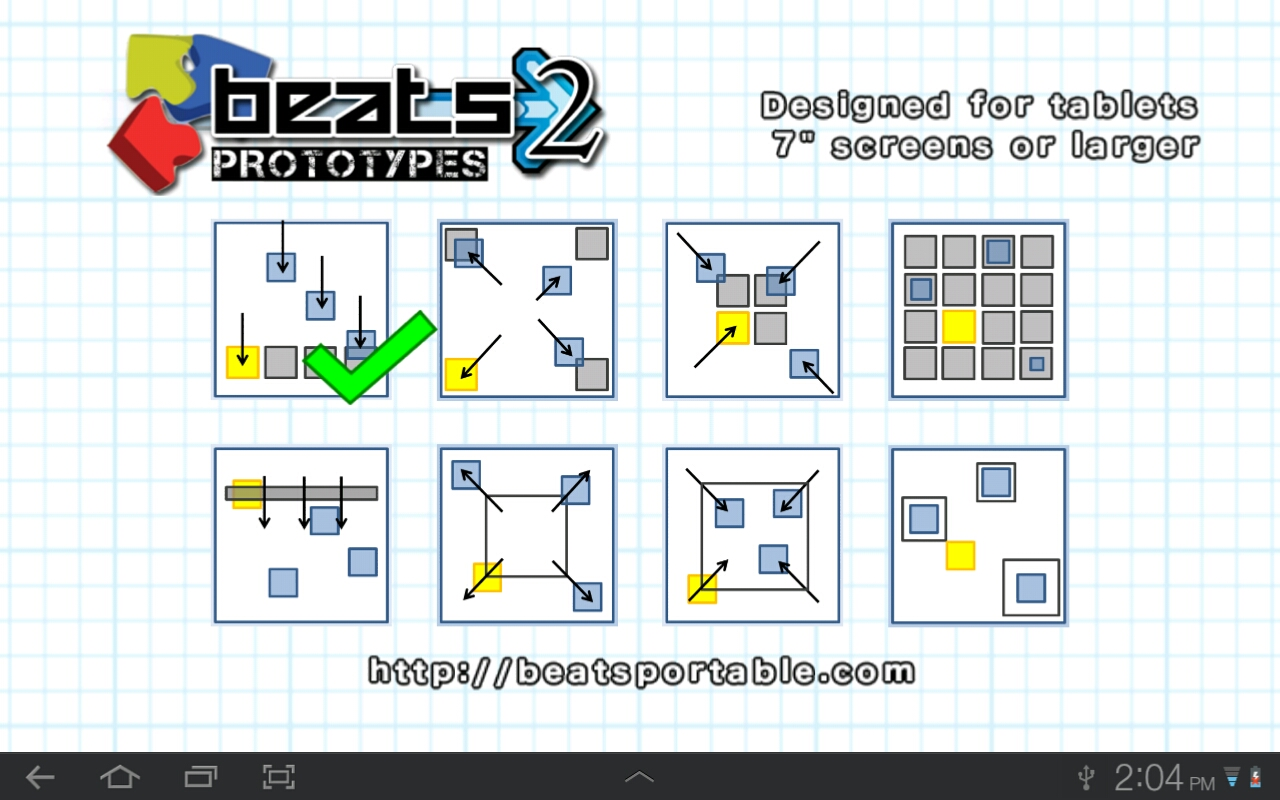
\includegraphics[width=1\linewidth]{figure_screenshot_main}
	\end{center}
	\vspace{-12pt}
	\caption{Screenshot of the ''Mode Select'' screen.}
	\label{fig:screenshot_main}
\end{figure}

In the ''Mode Select'' screen, all eight Modes will be displayed via their respective representative icons (see Figure~\ref{fig:screenshot_main}). Tapping on any of the icons will start the game featuring the respective Mode's interface design. For the user's convenience, gameplay history is kept for the duration of the session (launch to exit) and previously played Modes are indicated via an overlayed checkmark. \\

\noindent \textbf{Gameplay}

\begin{figure}[htb!]
	\begin{center}
		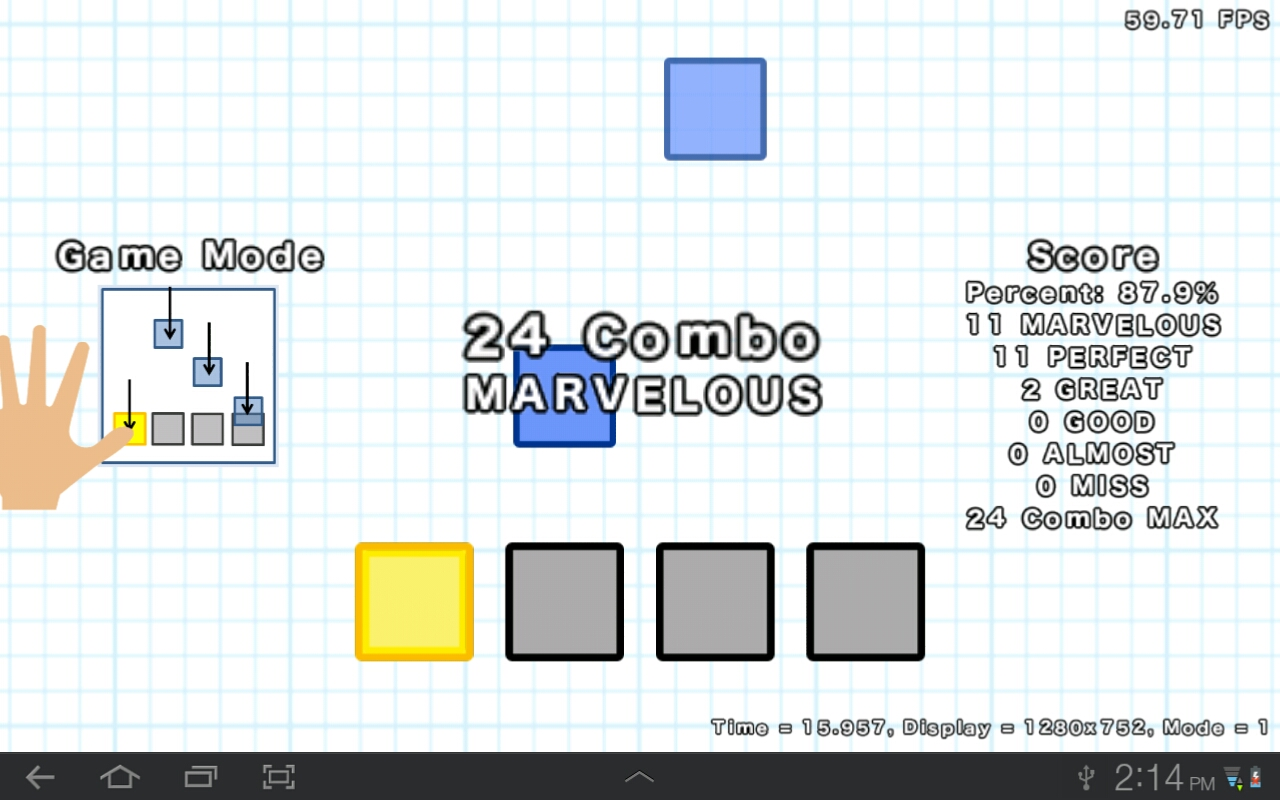
\includegraphics[width=1\linewidth]{figure_screenshot_gameplay_1}
	\end{center}
	\vspace{-12pt}
	\caption{Screenshot of Mode \#1's ''Gameplay'' screen.}
	\label{fig:screenshot_gameplay_1}
\end{figure}

\begin{figure}[htb!]
	\begin{center}
		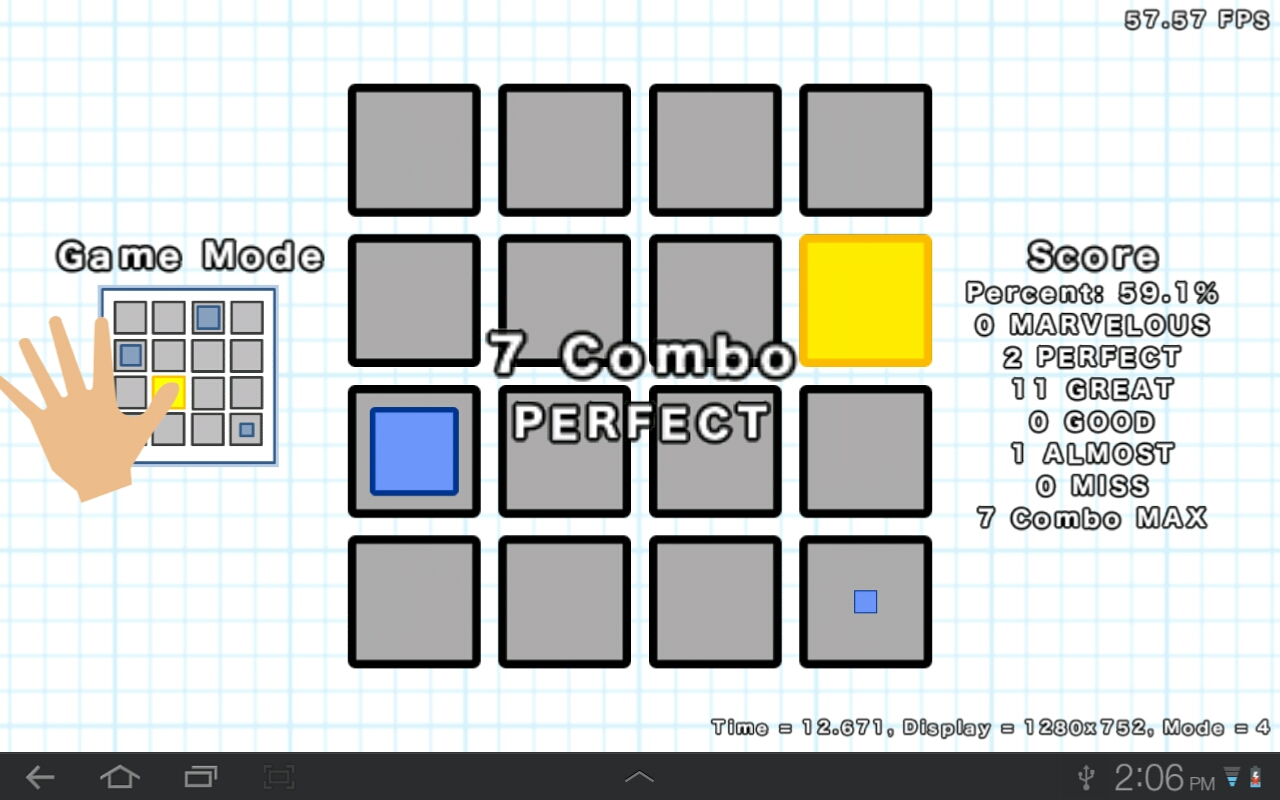
\includegraphics[width=1\linewidth]{figure_screenshot_gameplay_4}
	\end{center}
	\vspace{-12pt}
	\caption{Screenshot of Mode \#4's ''Gameplay'' screen.}
	\label{fig:screenshot_gameplay_4}
\end{figure}

After a Mode has been selected, the ''Gameplay'' screen loads (see Figure~\ref{fig:screenshot_gameplay_1} and ~\ref{fig:screenshot_gameplay_4}). For all eight Modes, the same common backend and data is used. The background song used was the rhythm game \textit{Beatmania IIDX 16: Empress}'s popular dance song ''smooooch'' by composer ''kors k''~\cite{smooooch}. The song was chosen for its strong, easy-to-recognize rhythm and steady, high tempo (177 BPM). The notes pattern data was generated using Karl O'Keeffe's open source program, \textit{Dancing Monkeys}, which generates note patterns with extremely high precision~\cite{dancing_monkeys}.\\

For all Modes, interface elements other than the notes and hitboxes were kept consistent. The left side of the screen featured the icon of the current Mode with an overlayed hand graphic indicating the suggested hand placement (explicit instructions would affect the ''Intuitive'' feedback metrics - see the \textit{Evaluation} section). The right side of the screen featured the current percent score and timing accuracy chart. The top right corner featured a live ''frames-per-second'' counter for debugging purposes. The bottom right corner featured a text label containing the current music time, the screen dimensions, and the current Mode, also for debugging purposes. The entire middle of the screen is an open square area in which the selected Mode's respective interface design is implemented. The only exceptions to this consistency are the location of the current combo and current accuracy text labels for Mode \#3, for which they were shifted underneath the hitbox area a bit to avoid obstructing view.\\

\newpage
\noindent \textbf{Score Updating}

While the game is running, notes are constantly loaded from the pre-generated notes pattern data and notes/hitbox properties updated. Whenever a note is hit, a score update event is triggered based on the timing accuracy of the note hit. Each note has its own corresponding expected time value (in milliseconds) which is compared to the current music time. The time difference is then compared against the chart in Figure ~\ref{fig:prototype_timings} to evaluate the qualitative timing accuracy value. For example, a time difference of 100ms (late) would map to a ''PERFECT'' note hit whereas 125ms would map to a ''GREAT'' note hit.

\begin{figure}[htb!]
	\begin{center}
		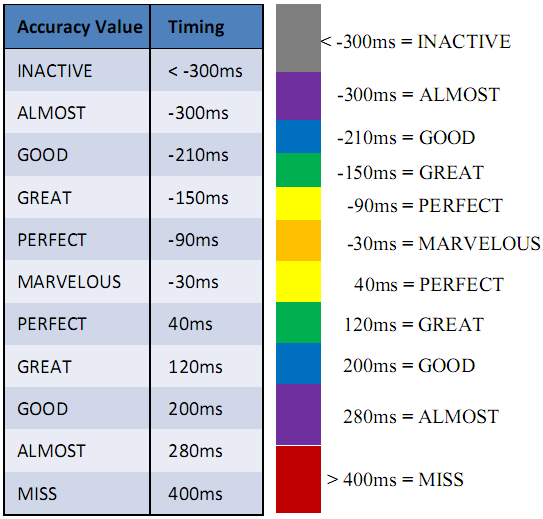
\includegraphics[width=1\linewidth]{figure_prototype_timings}
	\end{center}
	\vspace{-12pt}
	\caption{Timing chart used to evaluate a note hit's timing accuracy value.}
	\label{fig:prototype_timings}
\end{figure}

If the accuracy value is ''INACTIVE'', the note hit is ignored, otherwise, a respective counter is incremented. For accuracy values of ''GREAT'', ''PERFECT'' or ''MARVELOUS'', the combo counter is incremented. For other non-''INACTIVE'' values, the combo counter is reduced to zero. If the note ever reaches the ''MISS'' range, the miss event is automatically triggered (combo reduced to 0 and the ''MISS'' counter increases). Note that the accuracy value intervals in the positive range are greater than in the negative range to account for the observed tendency of users to hit notes slightly later.\\

The absolute value of the time difference is then added to a cummulative time difference sum and divided by the cummulative notes hit count to calculate the new percent score. A ''MISS'' is given the time difference of 400ms. Note that because the percent score is calculated with the raw time differences, two game playthroughs may have the same accuracy value counter numbers but slightly different percent scores. \\

After the accuracy value has been processed, the combo and accuracy text labels overlaying the middle of the screen and timing accuracy chart on the right side of the screen are then updated to reflect the new game statistics. \\

\newpage
\noindent \textbf{Feedback}

\begin{figure}[htb!]
	\begin{center}
		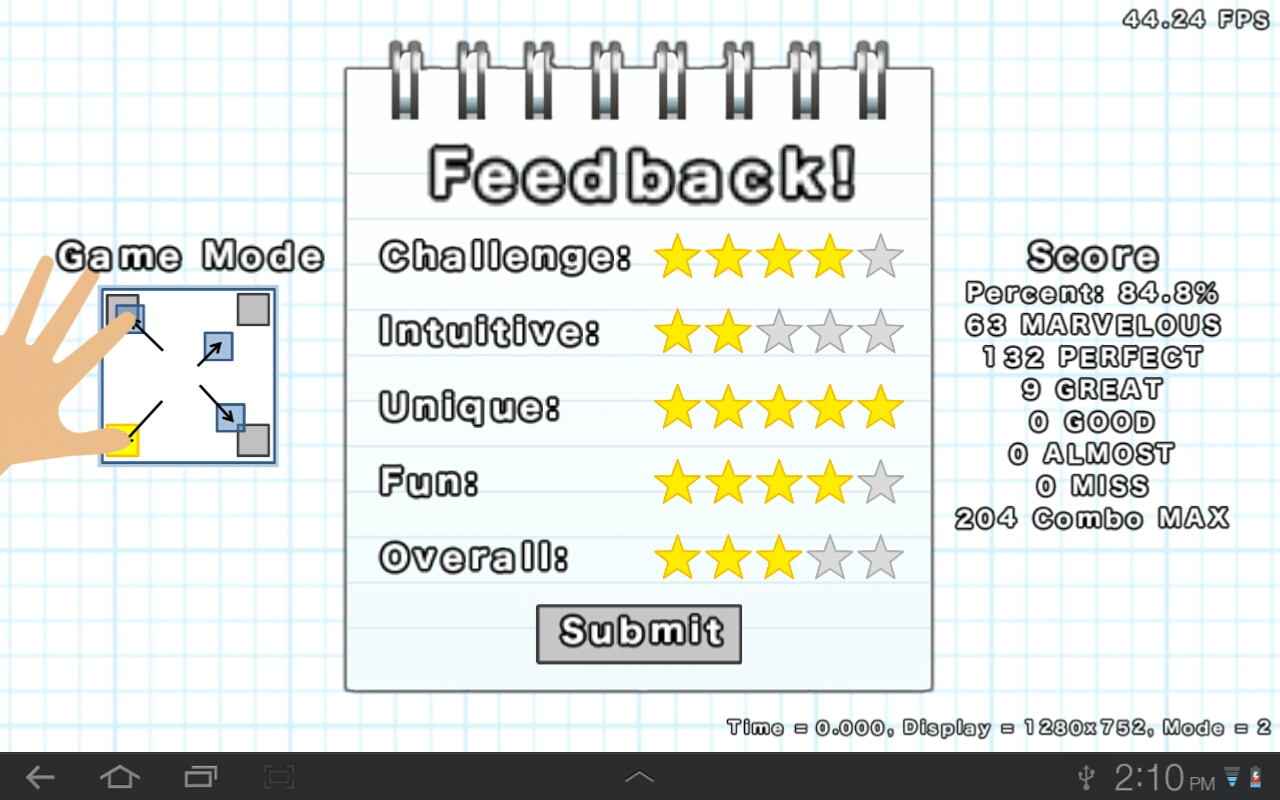
\includegraphics[width=1\linewidth]{figure_screenshot_feedback}
	\end{center}
	\vspace{-12pt}
	\caption{''Feedback'' overlay.}
	\label{fig:screenshot_feedback}
\end{figure}

Once the song is complete, the ''Feedback'' screen/overlay is displayed. The overlay presents an interface where the user can select a 1-5 star rating for each of the five feedback metrics (''Challenge'', ''Intuitive'', ''Unique'', ''Fun'', and ''Overall" - see the \textit{Evaluation} section for more details). Once all five of the categories have been rated, the ''Submit'' button becomes activated. Clicking on the ''Submit'' button will trigger tracker data sending, then bring the user back to the ''Mode Select'' screen.\\

\noindent \textbf{Data Tracking}

Upon the start of the gameplay, a ''Started'' event would be tracked and sent to \textit{Lumos}. Upon the completion of the gameplay, a ''Completed'' event would be tracked and the percent score, combo max value, and the entire timing accuracy chart's values would also be sent. Once the user completes the ''Feedback'' screen and taps the ''Submit'' button, the feedback ratings will also then be sent. Each tracked data is sent separately instead of together in the case that not all tracked data is available (e.g. the user exits the app without leaving feedback ratings). See the following \textit{Evaluation} section for more details on the data itself.

\subsection{Evaluation}
\label{subsec:project_outline}
In the \textit{Evaluation} stage of the study, the rhythm game prototype was published on \textit{Google Play}, the official app store for Android from Google~\cite{google_play}. A popular, previously published rhythm game, \textit{Beats, Advanced Rhythm Game}, was used to advertise the prototype~\cite{beats_portable}. The prototype app targetted tablet devices due to the facts that 1) Android tablets usually feature large multi-touch displays~\cite{honeycomb_tablet} for which interface design has a significant effect, and 2) Android tablet use is on the rise~\cite{tablet_use}. For comparison purposes, data collection was also done for Android phones, which feature a significantly smaller touchscreen.\\

To collect user data that can be used for this study, the app implemented a data tracker that uses a free metrics tracking service by \textit{Lumos} (see the \textit{Technical Resources} section for more details). Data was collected for quantitatively metrics (usage and gameplay statistics) and qualitative metrics (feedback ratings) for each individual Mode (\#1-8) and platform (tablet and phone).\\

\newpage
\noindent \textbf{Usage Statistics}

\vspace{+3pt}Usage statistics measured quantitatively:
\vspace{-3pt}\begin{itemize*}
	\item Game Started count\vspace{+3pt}
	\item Game Completed count\vspace{+3pt}
	\item Feedback Submitted count\vspace{+3pt}
\end{itemize*}

The usage statistics reflects on the overall prototype itself. Comparing the ''Game Started'' counts between the different Modes compares the popularity of each Mode relative to each other. A Mode that looks interesting at first look or is found to be interesting after the first playthrough will have a higher ''Started'' count. Comparing the ''Completed'' count to the ''Started'' count reflects on how well the Mode meets the user's expectations in interest level. A Mode that is boring and is not enjoyable to the user may not be played through to completion. The ''Feedback Submitted'' count can be used to calculate the percent of users who played through the Mode and was willing to provide feedback. These percentages can also be used as a rough measure of the accuracy of the results of this study.\\

\noindent \textbf{Gameplay Statistics}

\vspace{+3pt}Gameplay statistics measured quantitatively:
\vspace{-3pt}\begin{itemize*}
	\item Percent Score value\vspace{+3pt}
	\item Combo Max count\vspace{+3pt}
	\item MARVELOUS count\vspace{+3pt}
	\item PERFECT count\vspace{+3pt}
	\item GREAT count\vspace{+3pt}
	\item GOOD count\vspace{+3pt}
	\item ALMOST count\vspace{+3pt}
	\item MISS count\vspace{+3pt}
\end{itemize*}

The gameplay statistics reflect on the timing accuracy of the Mode being studied. A Mode with an interface design that is well suited for fast touch-based user input (e.g. playing rhythm games on a touchscreen devices) will inherently have gameplay statistics indicating high timing accuracy. The ''Percent Score'' value is a raw measure of this timing accuracy. The ''Combo Max'' count is correlated to the general consistency of timing accuracy. The specific accuracy value breakdown of hits gives a better picture of median average timing accuracy as ''Percent Score'' can be greatly skewed if the ''MISS'' count is high. Since Mode \#1's ''Falling Notes'' style is very common amoung currently available rhythm games, it is expected to have high familiarity amoung users and can be used as a baseline for comparison.\\

\noindent \textbf{Feedback Ratings}

\vspace{+3pt}Feedback ratings measured on a 1-5 star scale:
\vspace{-3pt}\begin{itemize*}
	\item Challenge\vspace{+3pt}
	\item Intuitive\vspace{+3pt}
	\item Fun\vspace{+3pt}
	\item Unique\vspace{+3pt}
	\item Overall\vspace{+3pt}
\end{itemize*}

These feedback ratings reflect on the game enjoyability of the Mode being studied. \\

The ''Challenge'' rating measures the difficulty of the gameplay. A high ''Challenge'' rating would imply that the user found the Mode's interface design difficult to use and react to, leading to low timing accuracy. A high ''Challenge'' rating could be either desirable or not depending on whether users see the difficulty as a nuisance or an added twist to the game; thus, this rating should be evaluated together with the ''Fun'' rating.\\

The ''Intuitive'' rating measures the learning curve of the gameplay. A high ''Intuitive'' rating would imply that the user found the interface easy to learn and easy to use. A user interface that feels natural and intuitive is usually highly desirable in games and allows for easier mastery (i.e. improved timing accuracy).\\

The ''Fun'' rating measures the direct enjoyability of the gameplay. Enjoyability is influenced by a number of possible factors depending on the user. For games where the goal is to have users enjoy spending time playing the game, a high ''Fun'' rating is desirable. \\

The ''Unique'' rating measures the novelty of the gameplay. In a competitive market where games often try to copy ideas off each other, originality and uniqueness can sometimes play an important factor in making a game stand out. A high ''Unique'' rating implies the user found the Mode very different from the rest, possibly as a new interface never used before. A unique game can draw many new users; however, it cannot predict the long-term success of the game. \\

The ''Overall'' rating measures the reception of the gameplay as a whole. A high ''Overall'' rating would imply that the user found the gameplay under that Mode to be suitable for a successful rhythm game, with all factors accounted for.

\section{Results}
\label{sec:results}

The following are results collected from the \textit{Evaluation} stage of the study. For each Mode, the average accuracy values are presented as pie charts for tablets and phones separately (see Figure~\ref{fig:data_accuracy} in the \textit{Appendix} for the complete data set), with the colour legend matching the colours used in timing diagram of Figure~\ref{fig:prototype_timings}. For analysis purposes here, a ''X\% accuracy'' refers to the combined percentage of accuracy values of ''PERFECT'' and ''MARVELOUS''.\\

The average feedback rating values are also presented as bar charts with tablet and phone data beside each other (see Figure~\ref{fig:data_rating} in the Appendix for the complete data set). The analysis, however, focused mainly on tablet data as most of the interfaces were not designed for the small screens of phones (defined in this study as having a screen size of under 5'' across). Specifically, the destination layout aspect is no longer an influential factor when the entire span of the screen is consistently in the user's viewing angle, thus requiring little change in focus. \\

In the last subsection, overall results were compared and Modes analyzed relative to each other. These results were then used to make general conclusions for each interface design in the \textit{Conclusion} section. Note that all analysis is only based on tablet results. \\

\newpage
\noindent \textbf{Mode \#1: Falling Notes}

\begin{figure}[htb!]
	\begin{center}
		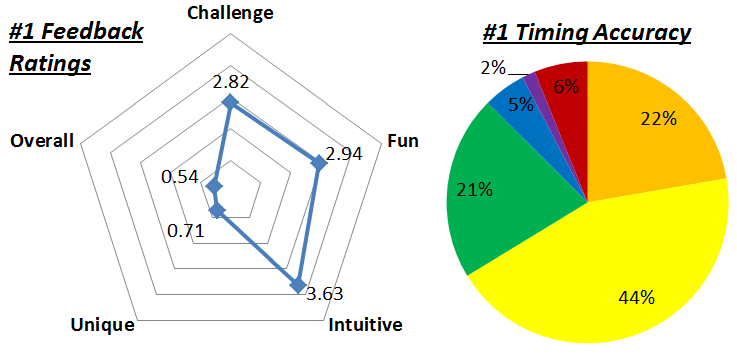
\includegraphics[width=1\linewidth]{figure_chart_1}
	\end{center}
	\vspace{-12pt}
	\caption{Mode \#1 data.}
	\label{fig:chart_1}
\end{figure}

Mode \#1 uses the ''Falling Notes'' style that is most common in rhythm games (see Figure~\ref{fig:interface_analysis}), so it can be used as a target baseline for the other Modes to try to match. Visual focus was at a fixed row of hitboxes, with notes moving along linear paths from the peripheral vision. The linear, overall single-dimensional direction of motion allows for more focus on accurate timing. As expected, accuracy was high at 66\%. \\

Mode \#1 received extremely low ''Unique'' and ''Overall'' ratings at 2.43 and 2.33 respectively. These low ratings can be attributed to the commonality of the style in rhythm games. \\

\noindent \textbf{Mode \#2: Spreading Notes}

\begin{figure}[htb!]
	\begin{center}
		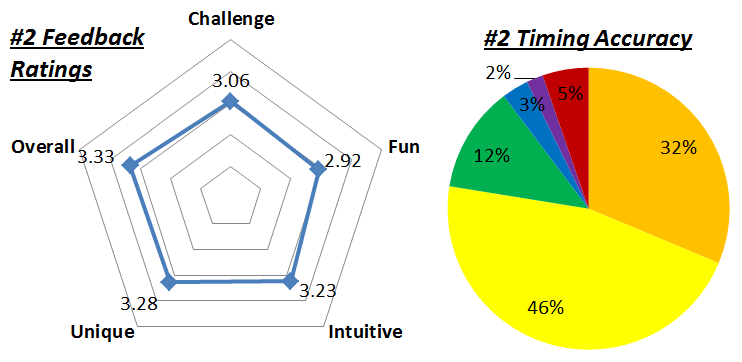
\includegraphics[width=1\linewidth]{figure_chart_2}
	\end{center}
	\vspace{-12pt}
	\caption{Mode \#2 data.}
	\label{fig:chart_2}
\end{figure}

Mode \#2 changes the visual focal points (from all on one side in Mode \#1) to the four corners of the screen. Since notes appear and move out from the centre, however, users could instead focus mainly there if the four corners still lie within peripheral vision (which is currently true for most touchscreen sizes). In addition, the corner hitbox placement means the hands can be placed around the perimeter of the tablet itself to avoid obstructing view of the notes. These positive factors are reflected in the results of an extremely high 78\% accuracy (surpassing Mode \#1).\\

Mode \#2 received strong ratings of almost 4.00 in all categories. \\

\newpage
\noindent \textbf{Mode \#3: Focusing Notes}

\begin{figure}[htb!]
	\begin{center}
		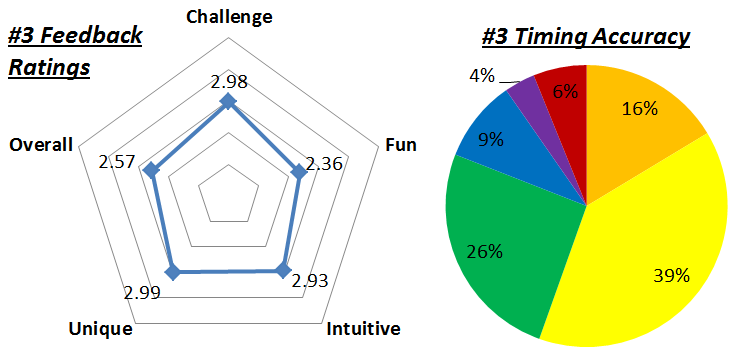
\includegraphics[width=1\linewidth]{figure_chart_3}
	\end{center}
	\vspace{-12pt}
	\caption{Mode \#3 data.}
	\label{fig:chart_3}
\end{figure}

Mode \#3 is the opposite of Mode \#2 in terms of focal position, with notes moving from the corners to a central location. While there is the advantage of tapping fingers only needing to travel short distances between hitboxes, the rest of the hand obstructs the screen. This disadvantage most likely explains the mediocre accuracy of 55\%. \\

Mode \#3 received relatively low ratings overall, with a low ''Fun'' rating of 3.42. \\

\noindent \textbf{Mode \#4: Grid}

\begin{figure}[htb!]
	\begin{center}
		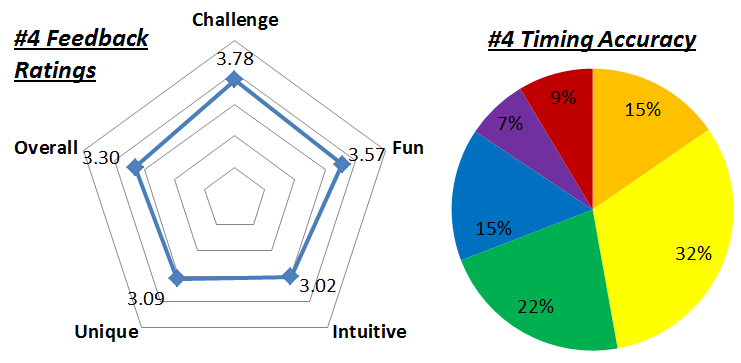
\includegraphics[width=1\linewidth]{figure_chart_4}
	\end{center}
	\vspace{-12pt}
	\caption{Mode \#4 data.}
	\label{fig:chart_4}
\end{figure}

Mode \#4's grid layout requires full focus on the entire screen, but at fixed points. The increased area of focus resulted in reduced focus per hitbox, leading to lower timing accuracy. The accuracy of this Mode was low at 47\%.\\

Mode \#4 received a high ''Challenge'' rating of 4.27, reflected in the low accuracy results. Despite this, the Mode was well received with ratings around 4.00 in the other four categories.\\

\newpage
\noindent \textbf{Mode \#5: Sliding Hitbox}

\begin{figure}[htb!]
	\begin{center}
		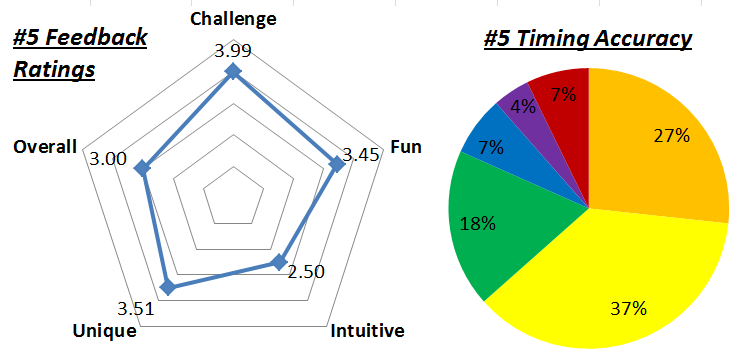
\includegraphics[width=1\linewidth]{figure_chart_5}
	\end{center}
	\vspace{-12pt}
	\caption{Mode \#5 data.}
	\label{fig:chart_5}
\end{figure}

Mode \#5  is the complement of Mode \#1 and shares the same advantage of having a single-dimensional direction of motion. Unlike Mode \#1, however, Mode \#5 requires the user to continuously change focus to follow the moving hitbox, moving from the bottom immediately back to the top. The resulting accuracy is good at 64\%. \\

Mode \#5 received a low 3.50 for ''Intuitive'' rating, most likely due to the game mode being uncommon. Although the Mode had high accuracy results, the high ''Challenge'' rating is possibly attributed to users finding the interface new and unintuitive at first. \\

\noindent \textbf{Mode \#6: Expanding Hitbox}

\begin{figure}[htb!]
	\begin{center}
		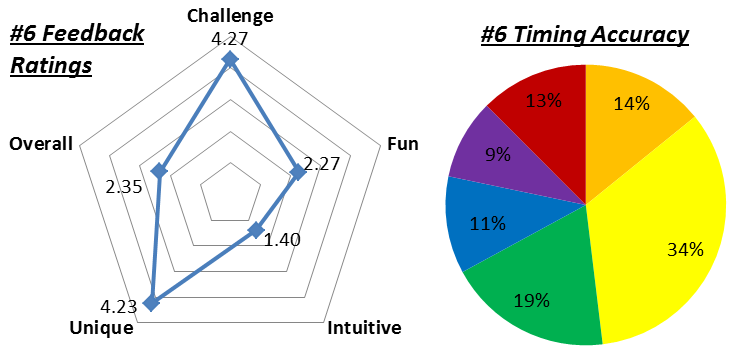
\includegraphics[width=1\linewidth]{figure_chart_6}
	\end{center}
	\vspace{-12pt}
	\caption{Mode \#6 data.}
	\label{fig:chart_6}
\end{figure}

Mode \#6  is the complement of Mode \#2. Unlike Mode \#2, however, the hitbox is not fixed, so the tapping fingers must continually move. Mode \#6 suffers the same disadvantage as Mode \#5 of a continously changing focus (from outside back to in). When tapping notes close to the centre, the same Mode \#3 vision-obstructing issue from hands applies. These compounded disadvantages lead to a poor accuracy of 48\%. \\

Mode \#6 received an extremely high 4.56 ''Challenge'' rating and a correspondingly low 2.84 ''Intuitive'' rating. While it has a high 4.54 ''Unique'' rating, the low ''Fun'' and ''Overall'' ratings indicates poor reception of the Mode. \\

\noindent \textbf{Mode \#7: Collapsing Hitbox}

\begin{figure}[htb!]
	\begin{center}
		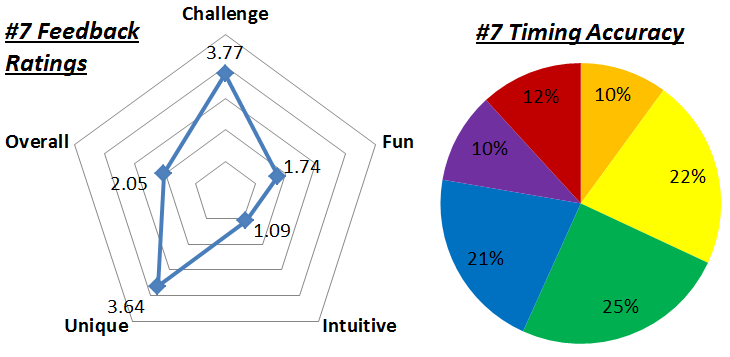
\includegraphics[width=1\linewidth]{figure_chart_7}
	\end{center}
	\vspace{-12pt}
	\caption{Mode \#7 data.}
	\label{fig:chart_7}
\end{figure}

Mode \#7 is the complement of Mode \#3. It shares all the disadvantages of Mode \#6 but with at a stronger level for vision-obstruction from hands. As a result, Mode \#7 has the lowest accuracy of all the Modes, at 32\% accuracy. \\

Mode \#7 received similar poor ratings to \#6, with the lowest ''Fun'' and ''Intuitive'' ratings of 3.04 and 2.65 respectively among all Modes. \\

\noindent \textbf{Mode \#8: Appearing}

\begin{figure}[htb!]
	\begin{center}
		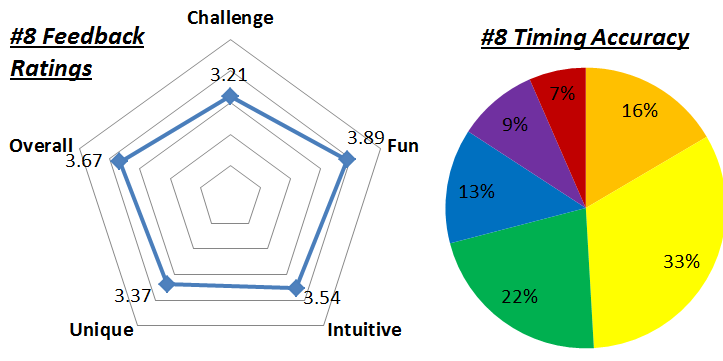
\includegraphics[width=1\linewidth]{figure_chart_8}
	\end{center}
	\vspace{-12pt}
	\caption{Mode \#8 data.}
	\label{fig:chart_8}
\end{figure}

Mode \#8 is the complement of Mode \#4. Because the hitboxes only appear when the note appears, however, the interface is a lot less cluttered, allowing for greater focus on the notes that do appear. The accuracy is slightly improved from Mode \#4 at 49\%. \\

Mode \#8 was very well received, with a ratings around 4.00 in all categories and the highest ''Fun'' rating of 4.33. \\

\newpage
\noindent \textbf{Overall}

\begin{figure}[htb!]
	\begin{center}
		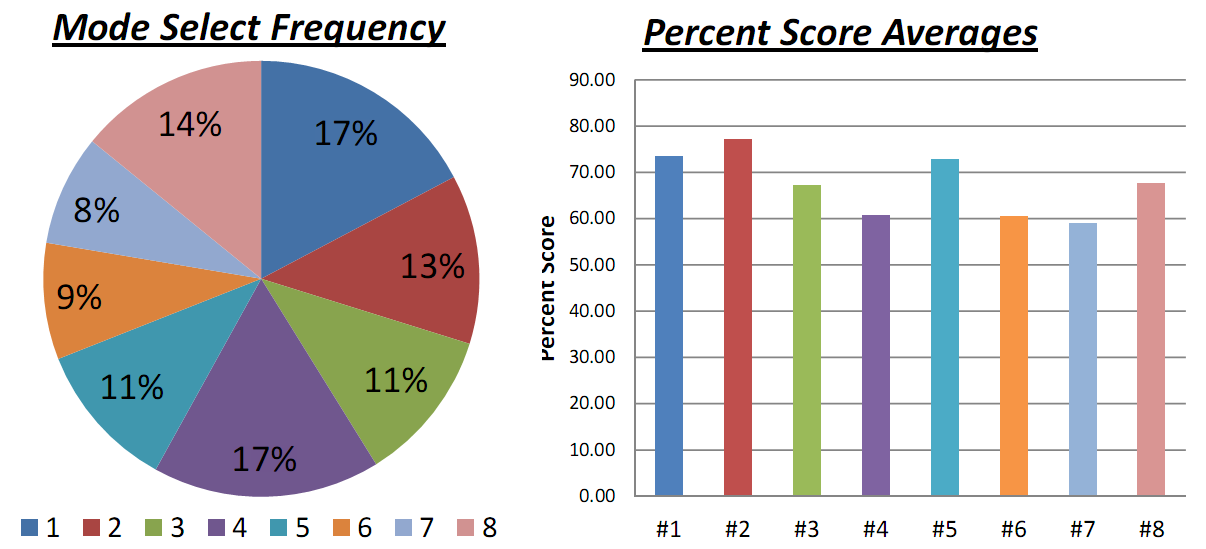
\includegraphics[width=1\linewidth]{figure_chart_overall}
	\end{center}
	\vspace{-12pt}
	\caption{Overall mode selection frequency and percent score averages.}
	\label{fig:chart_overall}
\end{figure}

Qualitatively, Modes \#2 and \#1 had the highest percent score averages, followed by \#5 and \#3 in that order. On the other hand, Modes \#6 and \#7 had extremely low percent scores and accuracy. This matches the relative accuracy percents determined from comparing each mode's accuracy value charts earlier.\\

Qualitatively, Modes \#8 was the best rated, receiving the highest ''Fun'' rating of 4.33 and around 4.00 for the other ratings. Mode \#2 was also very well received with almost 4.00 for all ratings. Mode \#1 received the lowest ''Unique'' and ''Overall'' ratings of 2.43 and 2.33 respectively, most likely due to its ''Falling Notes'' style being very commonplace and uninteresting. Despite that, it was also the most commonly played mode, with the highest mode select frequency of 17%. Modes \#6 and \#7 received very low ''Intuitive'' ratings of 2.84 and 2.65 respectively and also correspondingly low ''Fun'' ratings of 3.36 and 3.04 respectively.\\

\section{Conclusion}
\label{sec:conclusion}

In this study, two aspects of rhythm game successfulness are studied: timing accuracy and game enjoyability. Swetser and Wyeth argues that enjoyment of games does not only depend on the final outcome but also factors such as concentration, mastery, and fun~\cite{gameflow}. In this case, the final outcome is measured in timing accuracy via quantitative percent scores and accuracy charts, while the other factors are measured by game enjoyability via qualitative feedback ratings. \\

Because of the independence of these two aspects, two different concluding results can be made. When considering timing accuracy, Modes \#1 and \#2 are great choices, \#3 and \#5 are good choices, \#4 and \#8 are poor choices, and \#6 and \#7 are bad choices. When considering game enjoyability, Modes \#2, \#4 and \#8 are great choices, \#5 is a good choice, \#1 and \#3 are poor choices, and \#6 and \#7 are bad choices. These results are shown visually in Figure~\ref{fig:chart_results}.

\begin{figure}[htb!]
	\begin{center}
		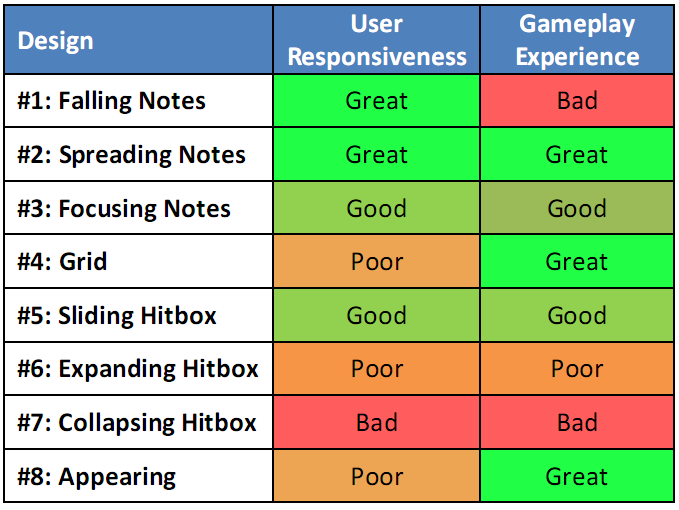
\includegraphics[width=0.9\linewidth]{figure_chart_results}
	\end{center}
	\vspace{-12pt}
	\caption{Comparing timing accuracy and game enjoyability of the studied rhythm game Modes.}
	\label{fig:chart_results}
\end{figure}

\section{Ethics}
\label{sec:ethics}
When using analytics services for mass data collection from users of software, privacy and unnecessary information collection is always a potential ethical concern. This study, unfortunately, is no exception. \\

For the \textit{Evaluation} stage of this study, user data is collected through \textit{Lumos}, an analytics service and associated software package written by Rebel Hippo Inc. (see the \textit{Technical Resources} section). While \textit{Lumos} is able to successfully collect data users of the app willingly submit for the sake of this study, it also automatically collects additional data about the device itself. Unnecessary but possibly privacy-infringing information such as the device's hardware specifications, OS details, and even locale is collected by default. While they are not relevant to this study, they do pass through an unaffiliated third party (Rebel Hippo Inc.). One possible solution to this potential risk would be to implement an in-house data collection service to replace the \textit{Lumos} setup.

\section{Future Work}
\label{sec:future_work}

On the game development side, the results of the game enjoyability comparisons of this study can be used for designing of more complex touch-based game interfaces. In particular, Modes \#2, \#4 and \#8 are strong candidates as starting points for interface designs of future rhythm games. The planned cross-platform ''Beats2, Advanced Rhythm Game'' will feature multiple game modes with designs based on those that proved popular in ''Beats2 Prototypes''~\cite{beats_portable}.\\

On the software development side, the results of the timing accuracy comparisons can be used in the designing of general user interfaces in other timing-sensitive applications. With touchscreens expected to become a prominent input method (a highly probably conclusion of current industry trends~\cite{information_display}), user interfaces for interacting with elements in time-critical scenarios will strongly benefit from designs targeting fast element recognition and reactivity. For example, research targetting military applications of touchscreens is still very active~\cite{army_mil}. In many military-related endeavours, a few milliseconds delay in reaction time can lead to drastically different results (e.g. selecting enemy targets or dodging enemy projectiles in combat). \\

On the interface research side, similar studies can be conducted comparing how these same interface designs perform in other specialized input settings. For example, a worthwhile future project would be modifying the prototype app to support \textit{Kinect} input and determining if the comparison results match. This can be accomplished through the \textit{KinVi 3D} project, which allows users to control a computer through a \textit{virtual} touchscreen powered by Microsoft \textit{Kinect} depth sensors~\cite{kinvi3d}. \\

\section{Technical Resources}
\label{sec:resources}

\vspace{4pt}

\noindent \textbf{Test Platforms} \\
The target touchscreen device for testing in this project was the Samsung Galaxy Tab 10.1. The Galaxy Tab is an Android tablet running on a 1GHz dual-core processor and has a 10.1-inch capacitive touchscreen~\cite{galaxy_tab}. A Samsung Captivate was also used to check phone compatibility. The Samsung Captivate is an Android phone running on a 1GHz single-core processor a 4-inch capacitive touchscreen~\cite{samsung_captivate}.\\

\noindent \textbf{Android SDK} \\
\url{http://developer.android.com/sdk/} \\
The \textit{Android SDK} is the set of development tools and core libraries required for developing Android applications. \\

\noindent \textbf{Unity3} \\
\url{http://unity3d.com/unity/publishing/android.html} \\
The \textit{Unity 3} development tools consists of the \textit{editor}, the series of tools for developing games, and the \textit{game engine}, the software backend that allows the developed games to run on target platforms. \textit{Unity 3} was chosen due to its cross-platform support of other touchscreen-supporting platforms and large community and professional support base. In this project, the prototype app runs on this game engine and was built for the Android target (as well as the PC target during development for debugging). The \textit{Unity3} license obtained for this project was the regular \textit{Unity3} package with the additional Android add-on to allow for development of Android apps. \\

\noindent \textbf{Lumos} \\
\url{http://www.uselumos.com/} \\
\textit{Lumos} is a free online service for tracking usage of features and other metrics. It is provided as an easily integratable \textit{Unity} package and was used in this study to collect user data for the \textit{Evaluation} stage. Because it is still a new service in development, however, the tracking servers are not always stable, leading to occasional request timeouts and thus loss of data. This can be seen in the occasional missing data points in the charts in the \textit{Appendix}. There currently is no other free, effective tracking service for \textit{Unity3} apps, however, and the missing data is weighed out through averaging existing data. \\

\noindent \textbf{ex2D} \\
\url{http://www.ex-dev.com/ex2d/} \\
\textit{ex2D} is a paid 2D framework for \textit{Unity3} game development. This was chosen over other alternatives (e.g. the free \textit{Othello 2D Framework} and the paid \textit{2D Toolkit}) due to its optimizations for mobile platforms, particularly rendering dynamic text. All graphical elements of the prototype app were created as ex2D sprite objects.

\section{Appendix}
\label{sec:appendix}
\textit{See figures on following pages.}

\bibliographystyle{plain}
\bibliography{prop_spec}

\begin{figure*}[htb!]
	\begin{center}
		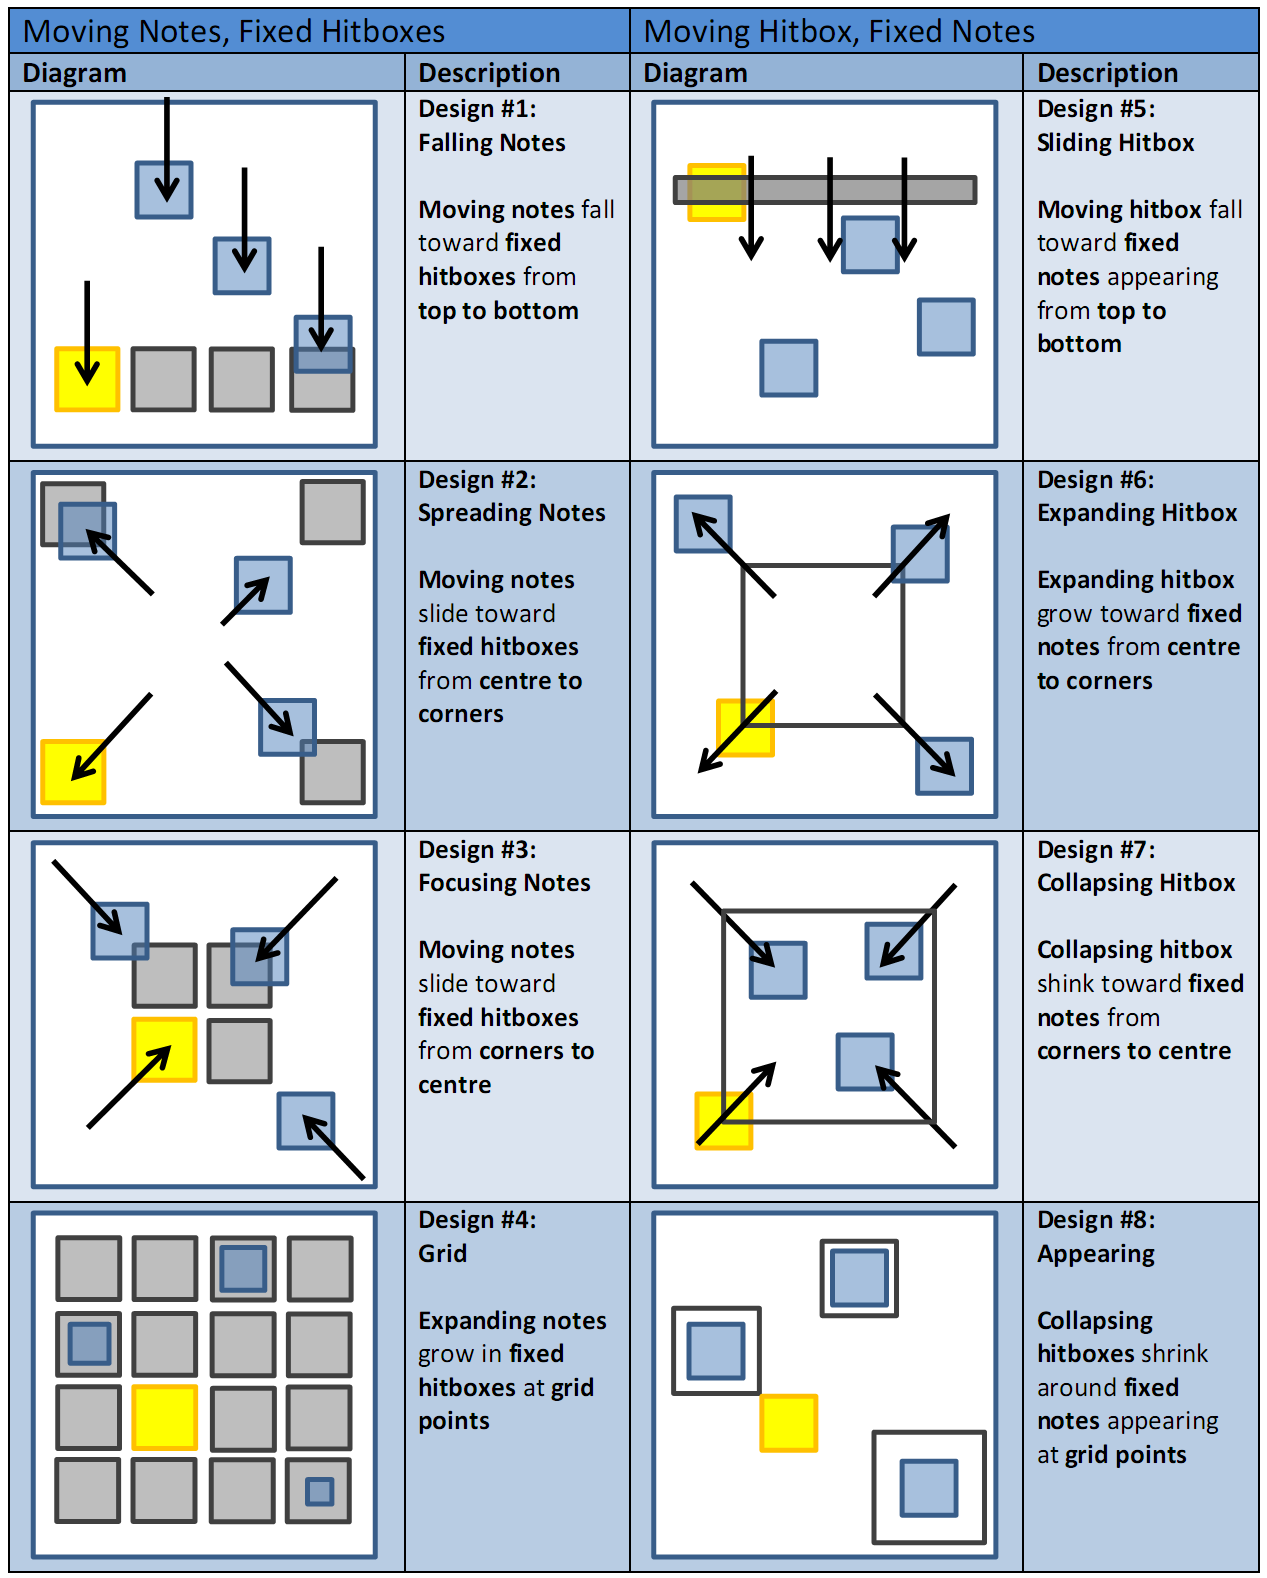
\includegraphics[width=0.9\linewidth]{figure_demo_interfaces}
	\end{center}
	\vspace{-12pt}
	\caption{Final interfaces designs (''Modes'') demoed in the final app.}
	\label{fig:demo_interfaces}
\end{figure*}

\begin{figure*}[htb!]
	\begin{center}
		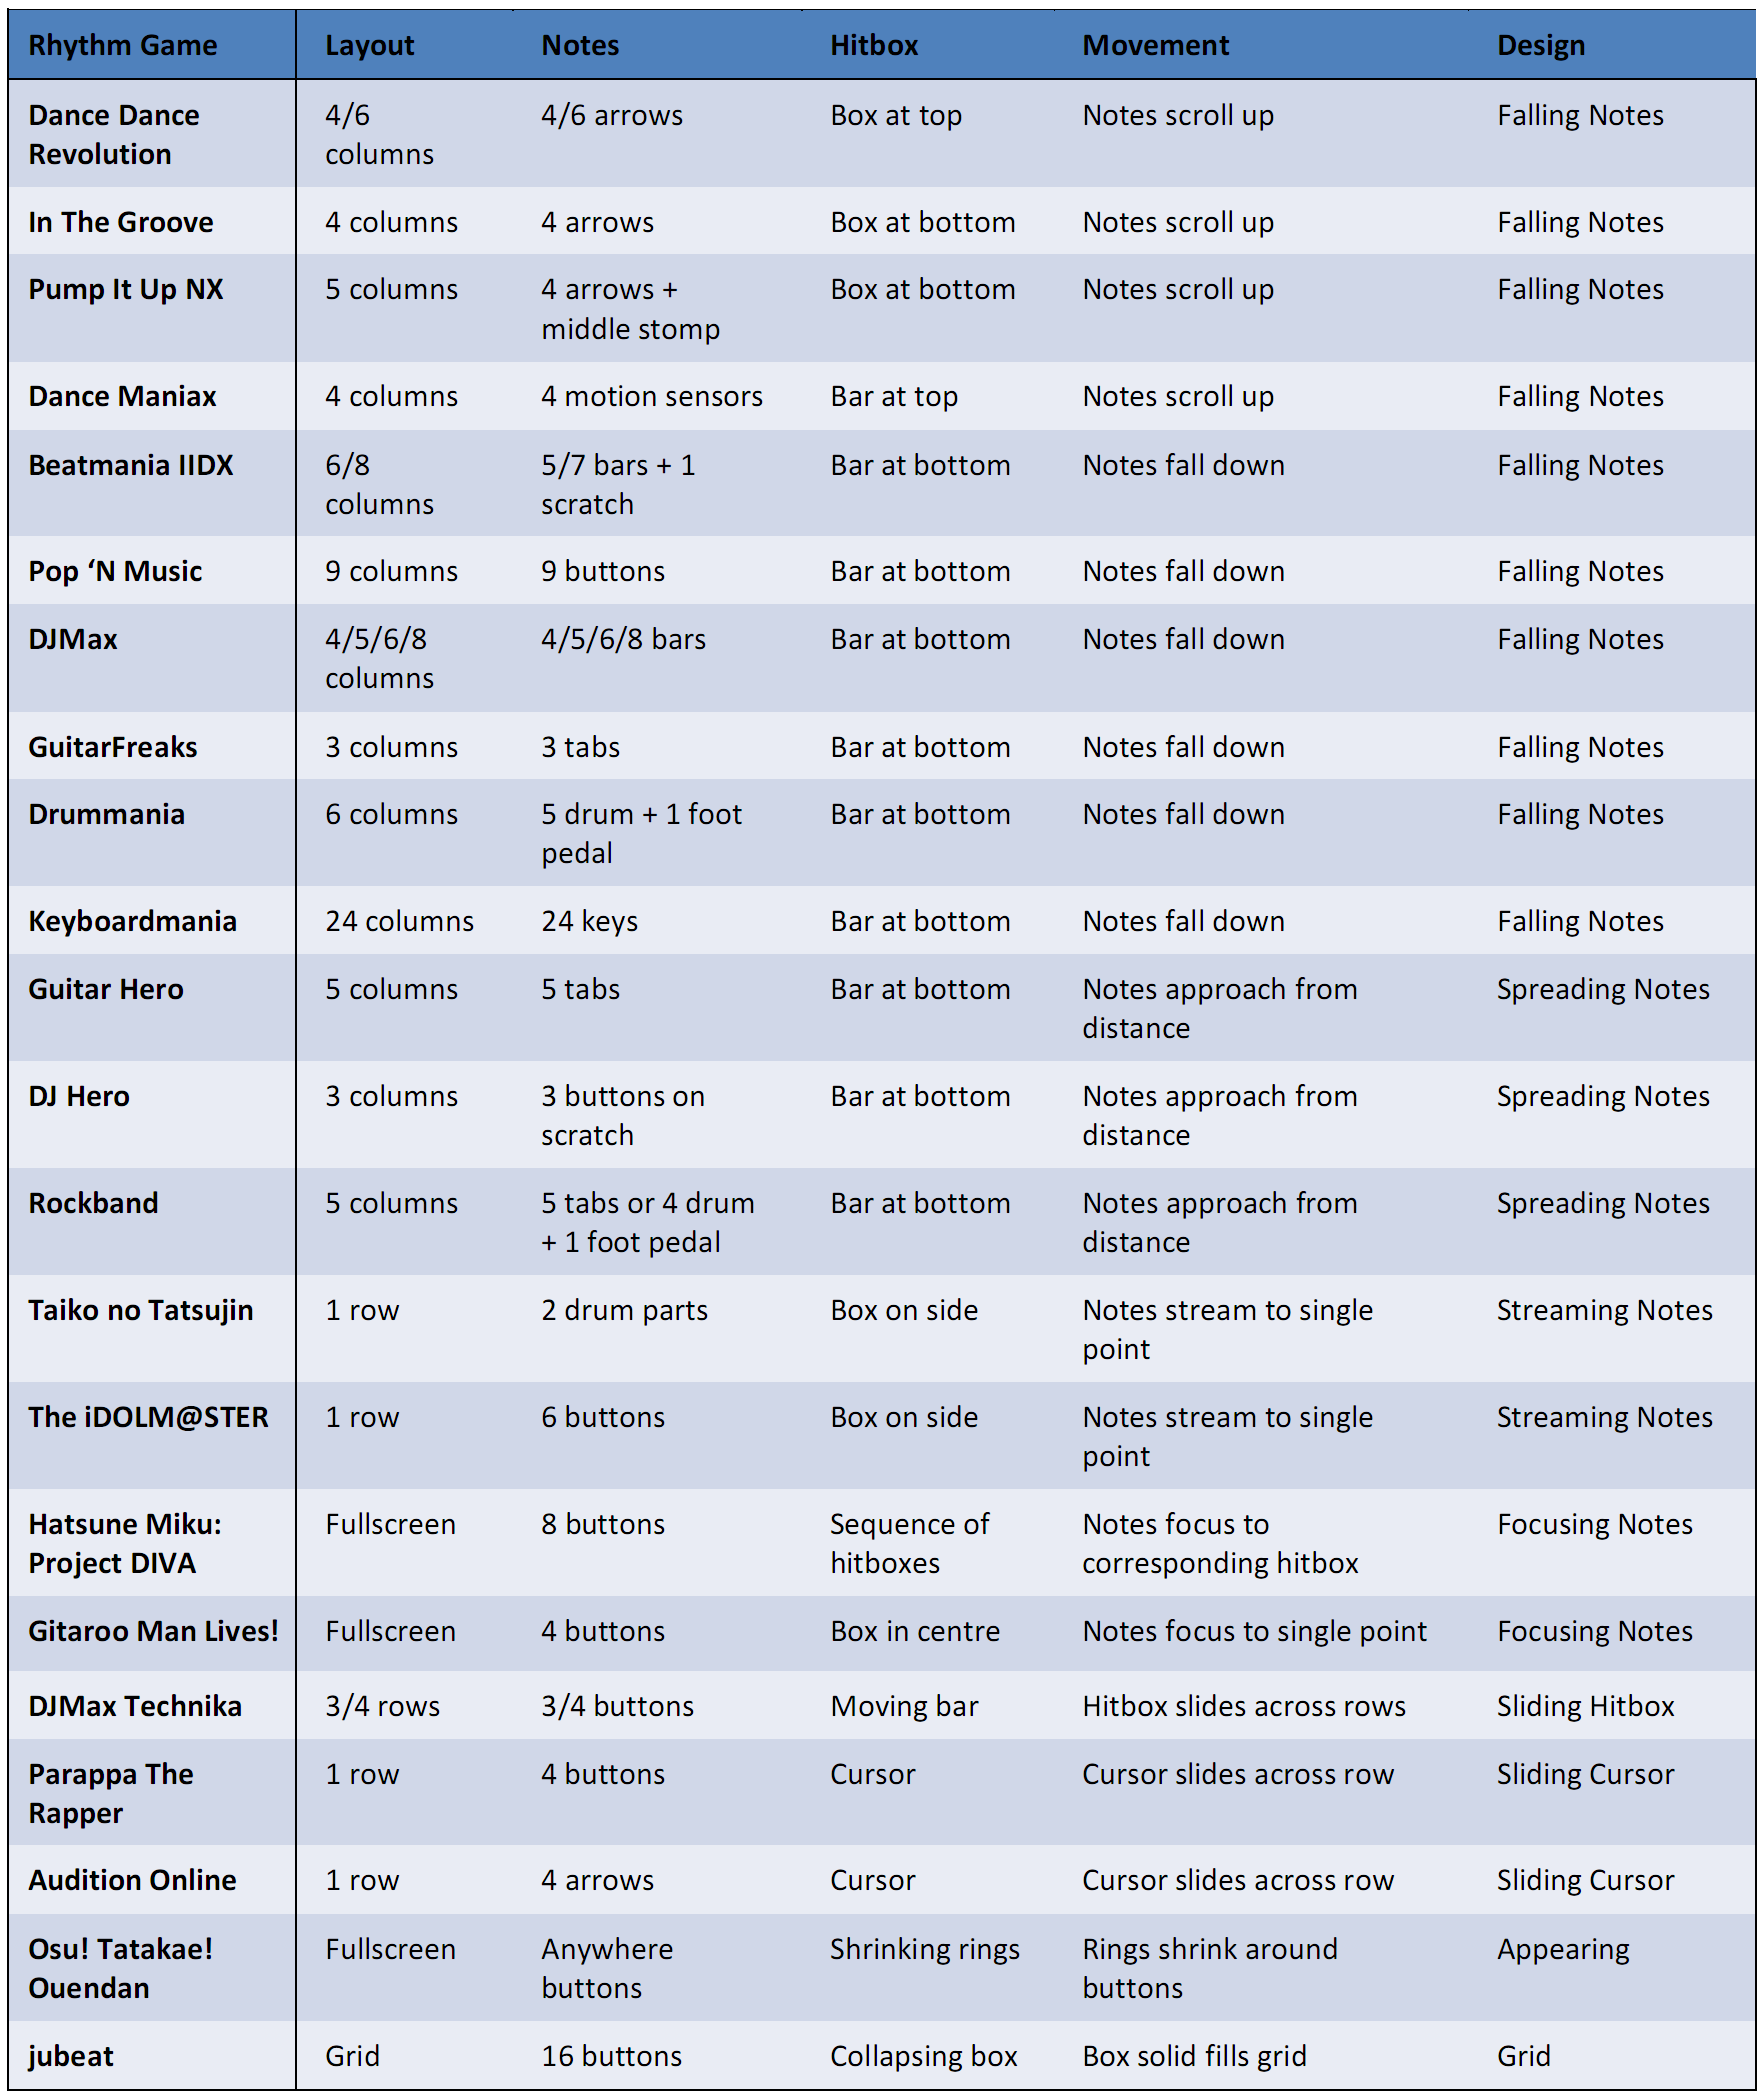
\includegraphics[width=1\linewidth]{figure_interface_analysis}
	\end{center}
	\vspace{-12pt}
	\caption{Analysis of the interfaces of various rhythm games.}
	\label{fig:interface_analysis}
\end{figure*}

\begin{figure*}[htb!]
	\begin{center}
		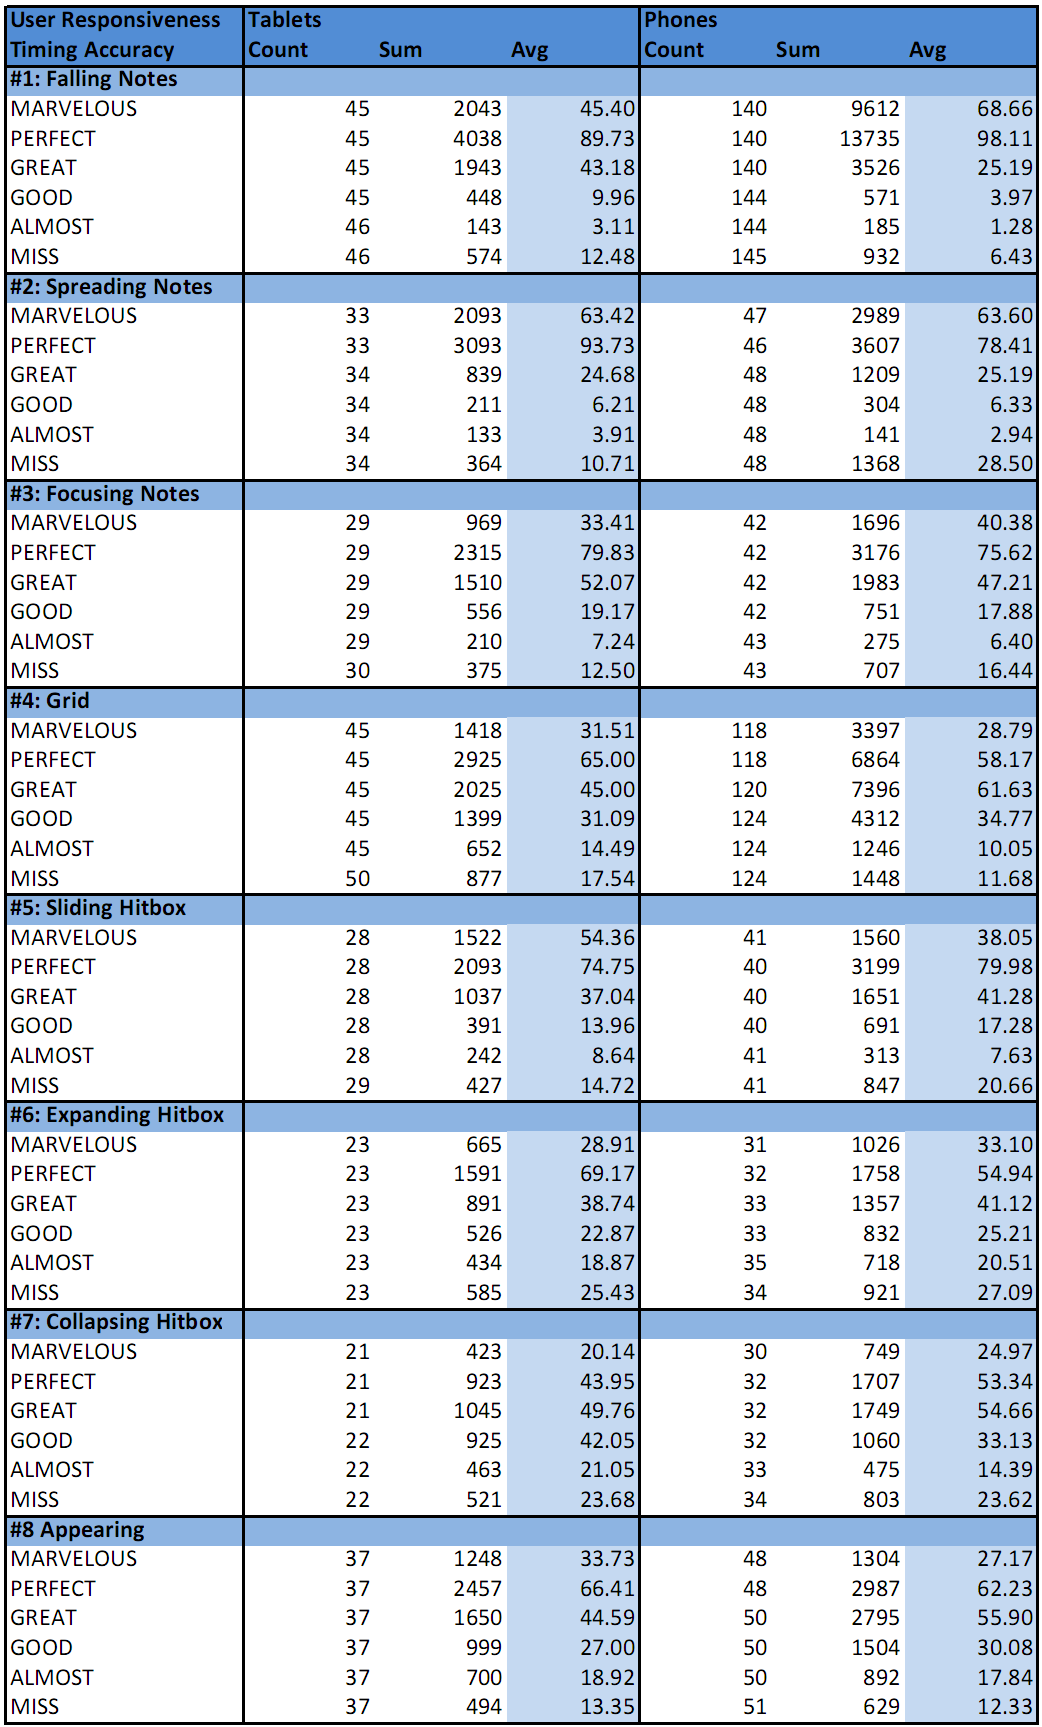
\includegraphics[height=1.1\textheight]{figure_data_accuracy}
	\end{center}
	\vspace{-12pt}
	\caption{Collected data on note accuracy counts for each mode.}
	\label{fig:data_accuracy}
\end{figure*}

\begin{figure*}[htb!]
	\begin{center}
		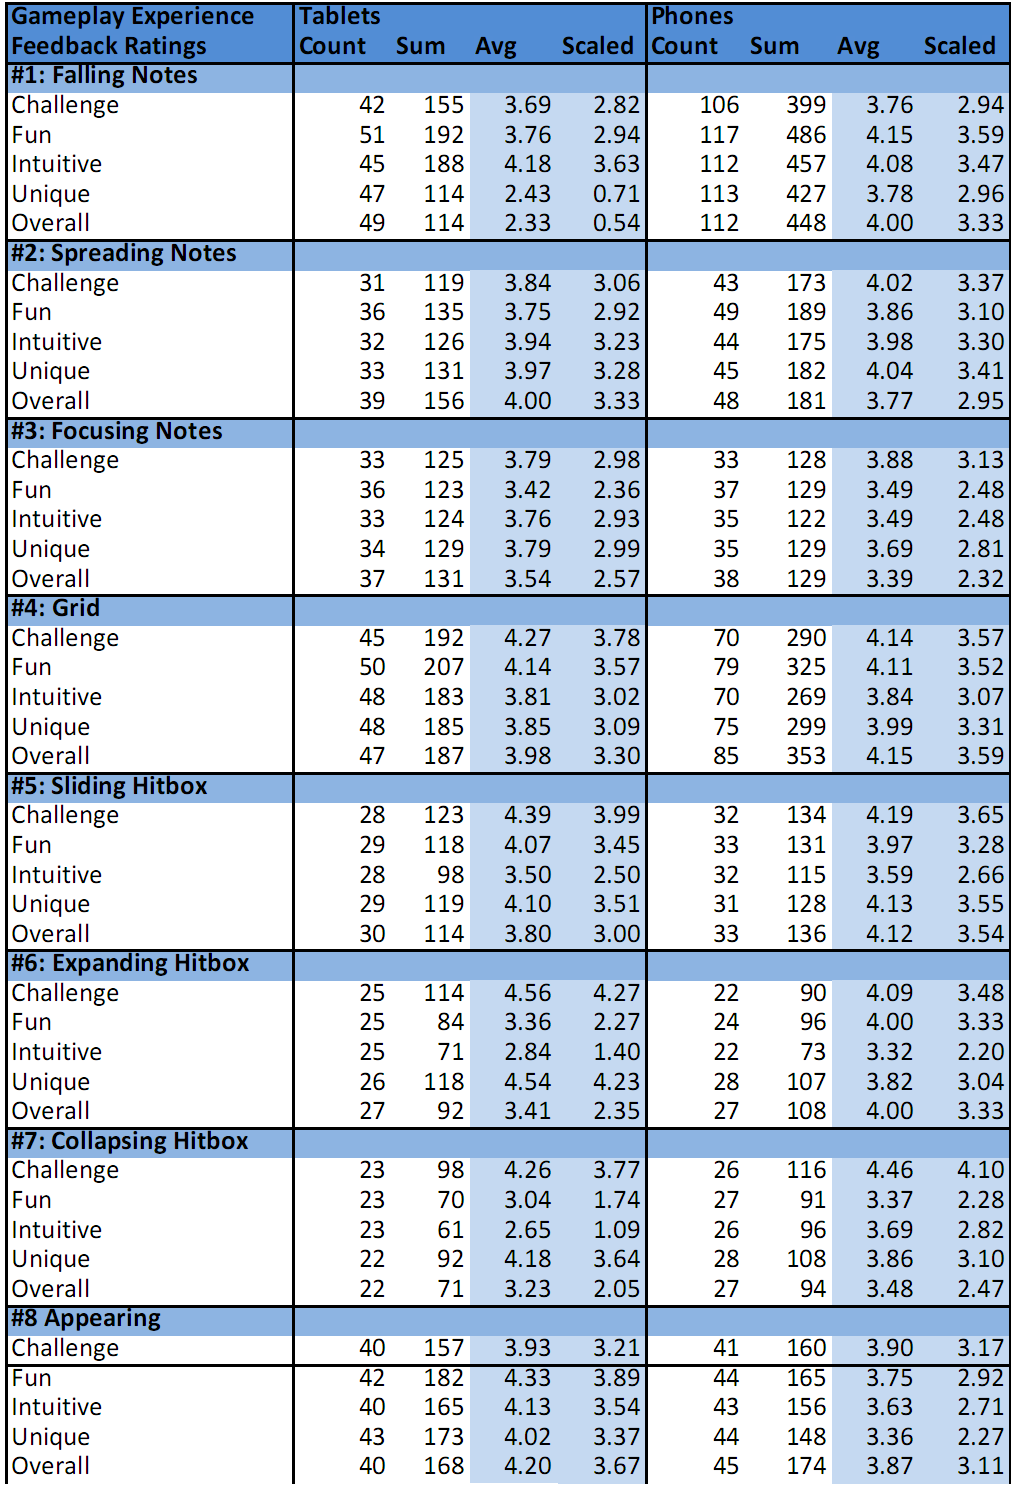
\includegraphics[width=0.9\linewidth]{figure_data_rating}
	\end{center}
	\vspace{-12pt}
	\caption{Collected data on feedback ratings for each mode.}
	\label{fig:data_rating}
\end{figure*}

\begin{figure*}[htb!]
	\begin{center}
		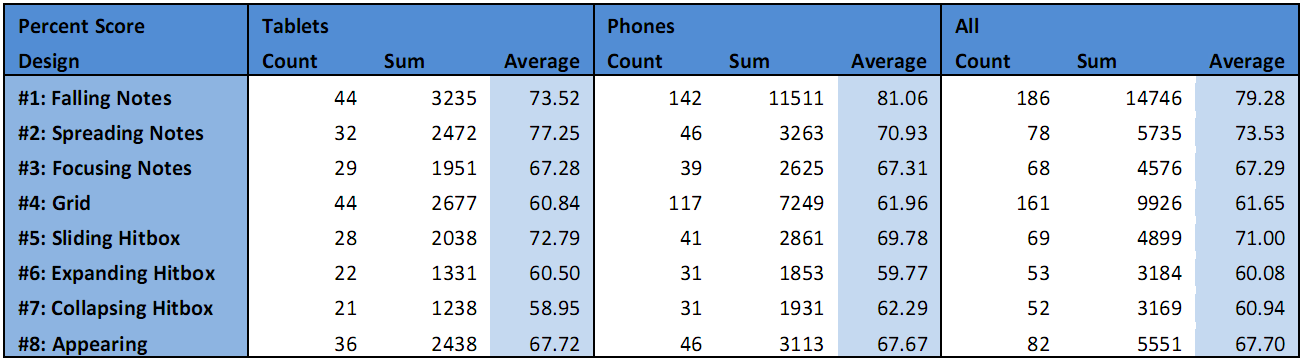
\includegraphics[width=1\linewidth]{figure_data_score}
	\end{center}
	\vspace{-12pt}
	\caption{Collected data on overall percent scores for each mode.}
	\label{fig:data_score}
\end{figure*}
\begin{figure*}[htb!]
	\begin{center}
		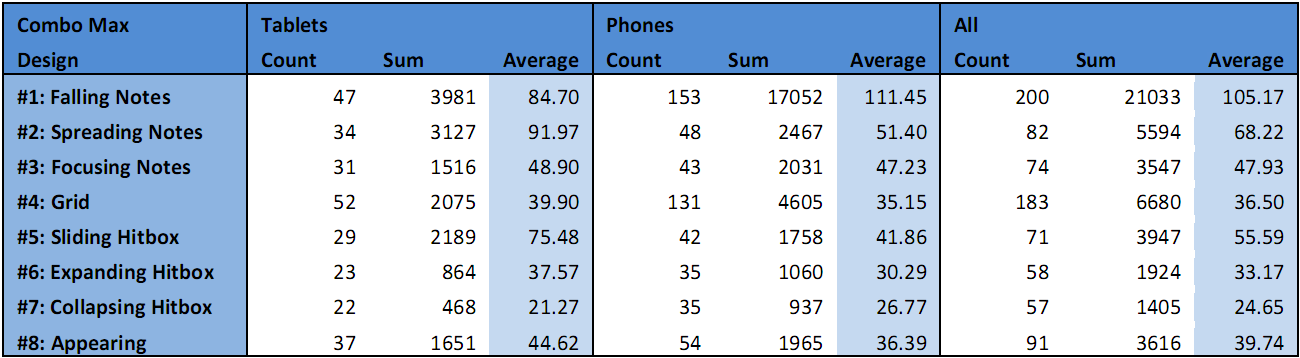
\includegraphics[width=1\linewidth]{figure_data_combo}
	\end{center}
	\vspace{-12pt}
	\caption{Collected data on ''COMBO MAX'' counts for each mode.}
	\label{fig:data_combo}
\end{figure*}
\begin{figure*}[htb!]
	\begin{center}
		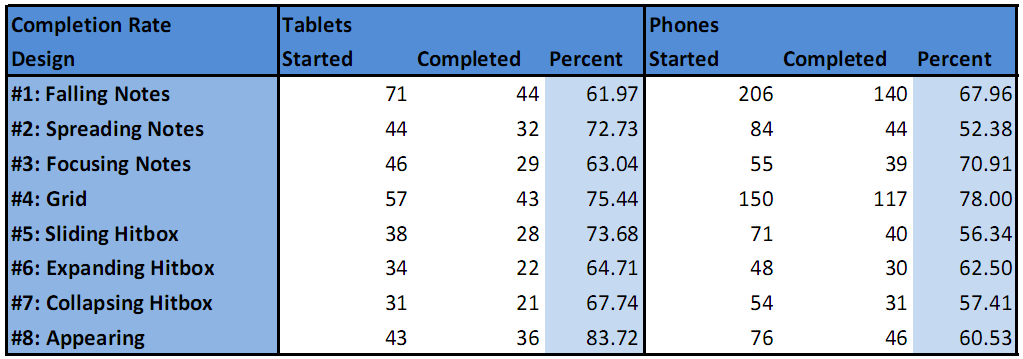
\includegraphics[width=1\linewidth]{figure_data_completion}
	\end{center}
	\vspace{-12pt}
	\caption{Collected data on completion rate for each mode.}
	\label{fig:data_completion}
\end{figure*}

\end{document} 

